\documentclass[12 pt]{article}
\usepackage{amsmath,amstext,amsgen,amsbsy,amsopn,amsfonts,graphicx,geometry}
\renewcommand{\baselinestretch}{2}

\addtolength{\oddsidemargin}{-.25in}
\addtolength{\evensidemargin}{-.5in}
\addtolength{\textwidth}{0.75in}

\addtolength{\topmargin}{-.5in}
\addtolength{\textheight}{1in}

\begin{document}

\title{Using Radio Relics to Constrain the  \\ Dynamics of 1 RXS J0603.3+4214 \\ \\ \\}

\author{A Thesis Presented By \\ \\
Emily Quinn Finney \\ \\ \\ \\
To the Keck Science Department \\
of Claremont McKenna, Pitzer, and Scripps Colleges \\
In partial fulfillment of \\
The degree of Bachelor of Arts \\ \\
Senior Thesis in Physics \\}

\date{December 9, 2013}

\maketitle

\newpage

\section*{Abstract}

Galaxy clusters, the most massive gravitationally bound objects in the universe, provide an important setting for exploring the structure and interactions of matter in the cosmos. When galaxy clusters merge, there is ample opportunity to examine interactions between densely-packed halos of luminous and dark matter; thus, understanding the dynamics of merging clusters provides insight into understanding  properties of dark matter. This paper examines the galaxy cluster 1 RXS J0603.3+4214 (“Toothbrush Cluster”), incorporating information about the polarization of its associated radio relics into Monte Carlo simulations to constrain knowledge about its inclination angle, time since collision, and the velocity and separation distance between its subclusters. We find that the collision velocity, time since merger, and 3D separation between subclusters are well-constrained, which allows for more accurate analysis of the history of the merger. This type of constraint could be applied to a variety of merging systems. Additionally, this constraint may allow opportunity for exploring the validity of different models of dark matter.

\newpage

\section{Introduction}

The importance of galaxy clusters to observational cosmology has long been established.  Historically, because galaxy clusters are the densest objects in the universe's large-scale structure, their observed number density in the universe has been used to constrain certain cosmological models and to more fully understand the development of structure in the universe (Campanelli et al. 2012 \cite{Campanelli12}, Rozo et al. 2010 \cite{Rozo10}, Sartoris et al. 2012 \cite{Sartoris12}). In recent years, however, galaxy clusters (and particularly galaxy cluster mergers) have become an especially important laboratory for observational cosmology and particle astrophysics, since these dense and massive structures may yield invaluable information about the interactions between luminous and dark matter in relatively easily observable systems. 

\begin{table}[h]
\centering
\begin{tabular}{|l|l|} \hline
Material & \% Composition \\ \hline
Dark Matter & 78-85\% \\
Intracluster Gas & 11-14\% \\
Galaxies and Other Luminous Matter & 2-6\% \\
\hline
\end{tabular}
\renewcommand{\baselinestretch}{1}
\caption{Composition of a galaxy cluster (Bohringer 2010) \cite{Bohringer10}.}
\label{tab1}
\end{table}

\renewcommand{\baselinestretch}{2}
Dissociative galaxy cluster mergers provide especially useful insight into studies of dark matter. In a dissociative merger, when two gravitationally bound mass structures (in this paper, these groups are called “subclusters”) collide, the constituent galaxies and dark matter halos pass directly through the merger, since they are so sparse that a collision between any one of them is extremely unlikely. Intracluster gas, on the other hand, will interact with the surrounding intracluster medium and experience a significant drag force which strips the subcluster of much of its gas (ram pressure stripping), and thus the vast majority of each subcluster\'s gas remains near the center of the merger event, between the post-merger subclusters.

\begin{figure}[h]
\renewcommand{\baselinestretch}{1}
\caption{The basic merger scenario for the situation in which dark matter does not interact with itself. Turquoise indicates dark matter, red indicates intracluster gas, black spots indicate galaxies, and purple indicates a mix of galaxies, dark matter, and gas. Note that the dark matter and gas dissociate immediately after the merger (far right). Figure courtesy of David Wittman.}
\label{cdm}
\centering
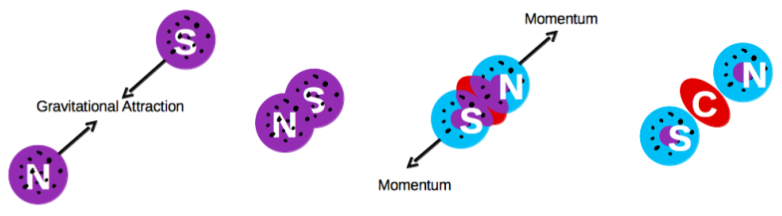
\includegraphics[width=0.8\textwidth]{cdm1}
\end{figure}

\renewcommand{\baselinestretch}{1}
Each of these components of a galaxy cluster (galaxies, dark matter, and intracluster gas) interacts with the other components gravitationally. Thus, when the galaxies and dark matter of one subcluster passes through those of another, it is gravitationally attracted both to the mass of the receding subcluster and to the intracluster gas in between the subclusters. Clearly, the center of the gravitational potential of the system is between the two subclusters. Then, as evident in Figure \ref{cdm}, the subclusters are gravitationally bound to the center of the merger. At a certain point, the subcluster's kinetic energy will be insufficient to continue traveling away from the center of the merger event, and the subcluster will thus begin returning to the center of the gravitational potential. Along the way, friction from intercluster gas and other forces (“dynamical friction”) deplete the system of kinetic energy and cause the subclusters to slow gradually. Even so, the system may oscillate for many millions of years before the kinetic energy is sufficiently dissipated to cause the system to dynamically relax.

This type of merger is ideal for studying the self-interaction of dark matter. If dark matter had a sufficiently large self-interaction cross section, it would interact with itself more strongly than would be expected by gravitational attraction alone; thus, we would expect some sort of offset between self-interacting dark matter and luminous matter (which only interacts with dark matter gravitationally). By determining the offset between the dark matter and luminous matter in a dissociative merger, the strength of the interaction of dark matter with itself may be measured and thus the dark matter self-interaction cross-section may be constrained (Markevitch et al. 2004) \cite{Markevitch04} (Figure \ref{sidm}).

\renewcommand{\baselinestretch}{1}
\begin{figure}[h]
\caption{The basic merger scenario for the situation in which dark matter does interact with itself. As with figure \ref{cdm}, turquoise indicates dark matter, red indicates intracluster gas, black spots indicate galaxies, and purple indicates a mix of galaxies, dark matter, and gas. Dark matter and gas dissociate immediately after the merger, but there is also dissociation of galaxies and dark matter. Figure courtesy of David Wittman.}
\label{sidm}
\centering
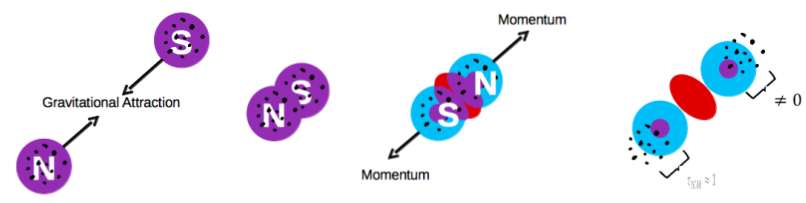
\includegraphics[width=0.8\textwidth]{sidm}
\end{figure}
\renewcommand{\baselinestretch}{2}

Thus, in order to examine the role of dark matter in galaxy cluster mergers, the dynamics of these mergers must be well-understood. Observational studies have traditionally analyzed galaxy cluster merger dynamics by invoking the timing argument (Barrena et al. 2002 \cite{Barrena02}, Girardi et al. 2008 \cite{Girardi08}, Boschin et al. 2012 \cite{Boschin12}), essentially looking at the extreme case in which two clusters begin colliding very far from each other (ie, the gravitational interaction between them is negligible), and are assumed to have a merger axis perpendicular to the line of sight. Several computational studies are more nuanced than this very simplistic timing argument approach, investigating parameters (time since collision, separation distance between subclusters, velocity of each subcluster, etc.) associated with known dissociative mergers. N-body hydrodynamical simulations (Skillman et al. 2013 \cite{Skillman13}, Vazza et al. 2011 \cite{Vazza11}) have proven to be useful, but require significant computational time; therefore, this paper invokes a Monte Carlo approach to examining the dynamics of galaxy cluster mergers (Dawson 2012 \cite{Dawson13}).

Within this approach, further data can be incorporated into an understanding of the attributes of galaxy cluster mergers, and some of this evidence comes in the form of long arcs of radio emission along one or both sides of the merger axis of some dissociative mergers (van Weeren et al. 2010 \cite{reinout10}, 2011b \cite{reinout11b}, 2011c \cite{reinout11c}, 2012 \cite{reinout12}). The leading contemporary theories postulate that these arcs are created by synchrotron emission from accelerated electrons during the shock of a collision of subclusters (Ensslin et al. 1998 \cite{Ensslin98}, Roettiger et al. 1999 \cite{Roettiger99}, Venturi et al. 1999 \cite{Venturi99}). This emission is polarized perpendicular to the direction of the magnetic field along which it occurs, so the degree to which an extended radio source appears polarized can constrain the angle at which the system is viewed. The magnetic fields within the intracluster gas of a merging galaxy cluster are usually quite disorganized, and when this gas is compressed during a shock, the magnetic fields can be aligned perpendicular to the line of sight of the merger axis but remain disorganized along the line of sight. Then if a system's radio relics display a high polarization fraction, it can limit the system to having a viewing angle nearly perpendicular to the line of sight. In this manner, the degree of polarization (which is strongly affected by the disorganization of the magnetic fields) can be used to provide an upper bound on the viewing angle of the magnetic field (Ensslin et al. 1998 \cite{Ensslin98}, van Weeren et al. 2011c \cite{reinout11c}, Skillman et al. 2013 \cite{Skillman13}).

In this work, the the radio relics around the merging galaxy cluster 1 RXS J060313.4+421231 (the “Toothbrush Cluster”) are examined and incorporated into previously established dynamical models of this cluster. The spectral index and polarization values of the radio relics associated with this cluster are used as priors in a Bayesian analysis of the system in order to constrain the viewing angle, collision velocity, time since collision, and other relevant parameters. The paper will be organized as follows: Section 2 examines the historical background of this project (Section 2.1 examines the history of dissociative merger and radio relic studies and Section 2.2 examines the history of methods used to study these structures). The data on the Sausage and Toothbrush clusters and the code used to analyze each of them are described in Section 3. In Section 4, results are presented, and they are discussed and related to major issues in cosmology in Section 5. The paper is concluded with Section 6. 

\newpage
\section{Historical Background}
\subsection{Galaxy Clusters, Dissociative Mergers, and Radio Relics}

Eighty years ago, Zwicky (1933) \cite{Zwicky33} first noticed discrepancies between galaxy cluster behavior and observational results, and in 1978, Rubin \& Ford confirmed that these results could be explained by the existence of a non-luminous, gravitationally-interacting substance adding mass to galaxies \cite{Rubin78}. This “dark matter” has been the subject of study for decades since, and although much progress has been made in cataloging its effects on various systems in the universe, little is understood about dark matter itself. Experimental studies of dark matter have historically explored two types of research: direct detection of dark matter using particle accelerators (CDMS \cite{CDMS}, LUX \cite{LUX}, XENON \cite{XENON}, CoGeNT \cite{cogent}, among many others) and indirect detection of dark matter in astrophysical situations. Direct detection studies have narrowed the mass values that dark matter particles could exhibit, and indirect detection studies allow structures of dark matter to be explored on a large scale (ie, Dietrich et al. 2012 \cite{Dietrich12}). Additionally, although it seems to be limited to gravitational interactions with luminous matter, it is still possible that dark matter could interact with itself in a measurable way (self-interacting dark matter, or SIDM); for this reason, several studies have focused on narrowing the possible values for the dark matter self-interaction cross-section (Clowe et al. 2006 \cite{Clowe06}, among others).

In this era of strong interest in the nature of dark matter, astrophysical systems provide a unique laboratory for investigating this unknown substance. Galaxy clusters provide a blend of dark and luminous matter that can be easily separated in a direct collision; the separation of these components could allow strong constraints on the properties of dark matter to emerge. More pertinently, since dark matter has yet to be identified and isolated on Earth, dissociative galaxy cluster mergers are one of the astrophysical laboratories in which dark matter self-interaction cross-sections could feasibly be studied. Dissociative merging galaxy clusters are defined as mergers in which two or more similarly-massive subclusters pass directly through each other, demonstrate measurable post-impact separation between galaxies, intercluster gas, and dark matter, and which occur at an angle nearly perpendicular to the line of sight for ease of observing this separation of components (Dawson et al. 2012 \cite{Dawson12}). Mergers that fit these criteria are relatively rare, since there exists only a small window between the time of initial impact of the two subclusters and the the time at which the system has reached equilibrium (ie., it is “dynamically relaxed”). 

Dissociative merging clusters were first targeted for study with the discovery of the Bullet Cluster (1E0657-56). The Bullet Cluster was first observed extensively by the infrared detector Chandra in October 2000 and first discussed as a merging system of interest by Markevitch et al. (2002) \cite{Markevitch02}, who noted that the system featured a very prominent bow shock (Figure \ref{bullet}).

\renewcommand{\baselinestretch}{1}
\begin{figure}[h]
\caption{Images of the Bullet Cluster, from Magellan (left) and Chandra (right). Green contours represent mass density as determined by weak gravitational lensing. Figure from Clowe et al. (2006) \cite{Clowe06}.}
\label{bullet}
\centering
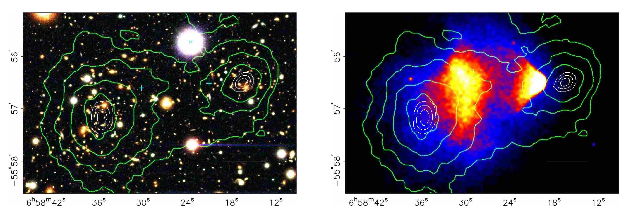
\includegraphics[width=0.8\textwidth]{cloweetal2006}
\end{figure}
\renewcommand{\baselinestretch}{2}

The remarkable clarity of this shock (the “bullet”) lent strong evidence that the shock was being viewed edge-on, and the density and temperature profiles obtained from the X-ray images allowed Markevitch et al. to estimate the relative velocity of the merging subclusters, the time since the original collision of the subclusters, and (later) the ram pressure on the bullet. In 2006, Clowe et al. published weak lensing observations that demonstrated no difference in the center of mass of the dark matter and luminous galaxies of the system, constraining the dark matter self-interaction cross-section ($\sigma/m$) to be less that $1$ cm$^2/$g \cite{Clowe06}. They noted that with a better understanding of the dynamics of the Bullet Cluster (both through observation and simulation), this merging cluster system could provide an important laboratory for further constraining the self-interaction cross-section of dark matter.

This reasoning (first suggested by Spergel \& Steinhardt in 1999 \cite{Spergel99}) can be applied to many dissociative merger systems; thus, a search for more dissociative merger systems began. While multiple mergers were discovered in the ensuing years, the next dissociative merger (MACS J0025.4-1222) was not confirmed until 2008 by Bradac et al \cite{Bradac08}. As demonstrated in Table \ref{tab2}, the remaining dissociative mergers have been primarily discovered in the past two years, and may be found in various parts of the sky. Most have redshifts less than 0.5.

\renewcommand{\baselinestretch}{1}
\begin{table}
\begin{tabular}{|p{2in}|l|l|l|l|l|} \hline
\textbf{Merger Name} & \textbf{Year} & \textbf{RA} & \textbf{Dec} & \textbf{z} & \textbf{Confirmed By} \\ \hline
1E0657-56 & 2004 & 06:58:29.2 & +50:30:37 & 0.279 & Markevitch et al. \cite{Markevitch04} \\
MACS J0025.4-1222 (Baby Bullet) & 2008 & 00:25:30 & -12:22:45 & 0.58 & Bradac et al. \cite{Bradac08} \\
Abell 1240 & 2009 & 11:23:32.1 & +43:06:32 & 0.194 & Barrena et al. \cite{Barrena09} \\
Abell 2744 (Pandora) & 2011 & 00:14:19.5 & -30:23:19 & 0.308 & Merten et al. \cite{Merten11} \\
ZwCl0008.8+52.15 & 2011 & 00:11:25.6 & +52:31:41 & 0.10 & van Weeren et al. \cite{reinout11b} \\
Abell 520 & 2012 & 04:54:19.0 & +02:56:49 & 0.199 & Jee et al. \cite{Jee12} \\
Abell 1758 & 2012 & 13:32:32.1 & +50:30:37 & 0.279 & Boschin et al. \cite{Boschin12} \\
Abell 2163 & 2012 & 16:15:34.1 & -06:07:26 & 0.203 & Soucail  \cite{Soucail12} \\
Abell S1063 & 2012 & 22:48:54.3 & -44:31:07 & 0.347 & G{\'o}mez et al. \cite{Gomez12} \\
ACT-CL J0102-4915 (El Gordo) & 2012 & 01:02:00.0 & -49:15:00 & 0.75 & Menanteau et al. \cite{Menanteau12} \\
DLS-CL J0916.2-2951 (Musket Ball) & 2012 & 09:16:12 & +29:51 & 0.53 & Dawson et al. \cite{Dawson12} \\
MACS J0717+3745 & 2013 & 07:17:33.8 & +37:45:20 & 0.545 & Medezinski et al. \cite{Medezinski13} \\
ZwCl1234.0+2916 & 2013 & 12:36:10 & +28:59:00 & 0.22 & Dahle et al. \cite{Dahle13} \\
\hline
\end{tabular}
\caption{Confirmed dissociative galaxy cluster mergers, with the year of discovery, location in the plane of the sky, redshift, and group that confirmed discovery.}
\label{tab2}
\end{table}
\renewcommand{\baselinestretch}{1}

One element of interest in some galaxy cluster mergers is the presence of extended radio structures outside the center of the merger event. These radio arcs are often highly polarized (in some cases, up to 60\%, van Weeren et al. 2012 \cite{reinout12}) and usually fall between 0.5 and 1.5 Mpc from the center of the cluster (van Weeren et al. 2010 \cite{reinout10}, 2011c \cite{reinout11c}, 2012 \cite{reinout12}; Vazza et al. 2011 \cite{Vazza11}). Most often, these relics occur on only one side of a merger (“single relic”), but sometimes they may appear perpendicular to the merger axis on both sides of the merger (“double relic”). Skillman et al. (2013) proposed that radio relics are less likely to be found when merger subclusters have just collided (Figure \ref{skillman5}), so it is possible that the galaxy cluster mergers in our sample may be somewhat older mergers \cite{Skillman13}. 

\renewcommand{\baselinestretch}{1}
\begin{figure}[h!]
\caption{Change of type of radiation with time. Note that the radio emission peaks with gas density, and does not appear to be strong immediately after a merger occurs. Figure from Skillman et al. (2013) \cite{Skillman13}.}
\label{skillman5}
\centering
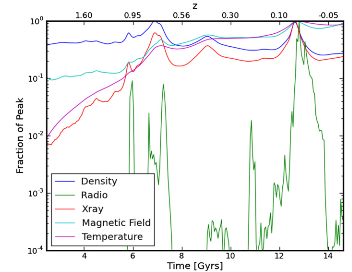
\includegraphics[width=0.5\textwidth]{skillman5}
\end{figure}
\renewcommand{\baselinestretch}{2}

While extended radio structures may occur in a variety of situations, structures that can be classified as “radio relics” must be long and somewhat narrow, and more importantly, must occur along the outside edge of a galaxy cluster merger (the other most common type of radio source, “radio halos”,  are characterized by diffuse emission occurring across the center of the merger). 

\renewcommand{\baselinestretch}{1}
\begin{figure}[h]
\caption{Simulation of radio emission at different viewing angles. The top right figure shows a completely edge-on viewing, and then viewing angles increase by $10^{\circ}$ for each image, from left to right and top to bottom. Figure from Skillman et al. (2013) \cite{Skillman13}.}
\label{skillman6}
\centering
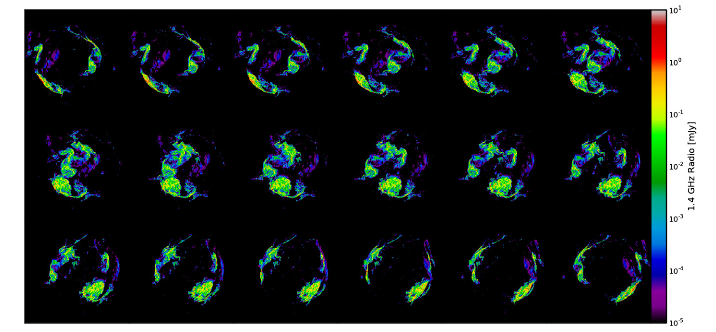
\includegraphics[width=0.8\textwidth]{skillman6}
\end{figure}
\renewcommand{\baselinestretch}{2}

The leading theory as to how these relics are formed is that during a galaxy cluster merger, intracluster gas clouds impact each other and produce a shock wave which emanates through the cloud. Since hot intracluster gas is comprised of charged particles, when these particles are accelerated, they induce a magnetic field oriented in one direction and synchrotron emission in another direction (Blandford \& Ostriker 1978 \cite{Blandford78}). The shock, however, compresses the intracluster gas (ie, the medium in which the electrons are accelerated) in one direction, allowing the electrons to move along the two dimensions perpendicular to the shock but limiting their motion along the direction of the shock propagation (Figure \ref{skillman6}). This causes the synchrotron emission to be more polarized perpendicular to the merger axis, although as evident in Figure \ref{skillman9}, the emission still appears to be disorganized when viewed face-on because electron motion can occur in two dimensions perpendicular to the shock propagation (Ensslin et al. 1998 \cite{Ensslin98}, Skillman et al. 2013 \cite{Skillman13}). 

\renewcommand{\baselinestretch}{1}
\begin{figure}[h!]
\caption{Polarization of a simulated radio relic at two resolutions (high resolution: top; low resolution: bottom). Polarization direction is shown with black lines, while polarization fraction strength is shown by color. The left panels denote an edge-on radio relic; the right panels denote a radio relic viewed face-on. Figure from Skillman et al. (2013) \cite{Skillman13}.}
\label{skillman9}
\centering
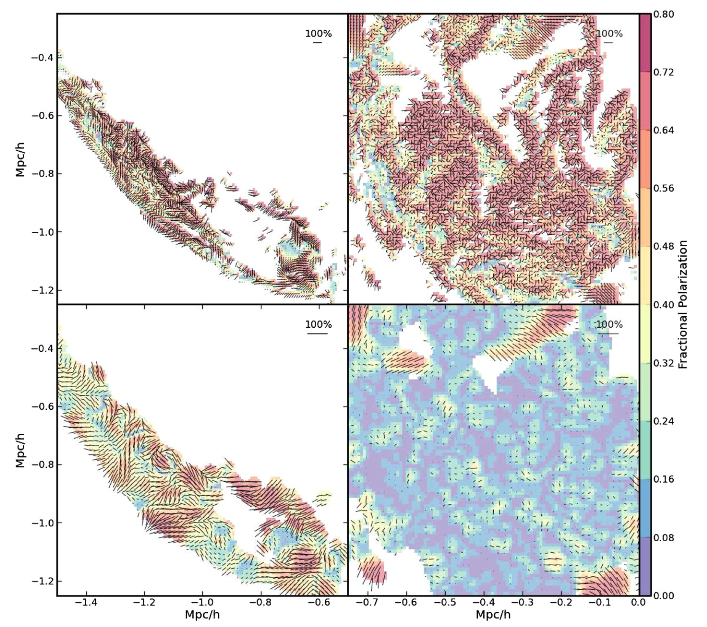
\includegraphics[width=0.8\textwidth]{skillman9}
\end{figure}
\renewcommand{\baselinestretch}{2}

\subsection{Methods Used to Analyze Merging Systems}

Several methods have been applied to the study of merging galaxy cluster dynamics. The first of these, commonly known as the “timing argument”, was not originally developed for studying merging galaxy clusters, but has proven useful to observational astronomers due to its simplicity and generalizability. The basic premise of this argument is to assume that a system of two masses is directly perpendicular to the line of sight, and to place the two point masses at a location at which they are observed. The point masses are subsequently permitted to interact gravitationally, with the assumption that rather than orbiting each other or passing around each other, eventually the distance between the point masses will be zero. Given these conditions, the locations of the point masses at any time can be solved by using Newtonian equations of motion (Peebles 1993 \cite{Peebles93}). Although this argument is frequently invoked, its simplicity also prohibits it from being a nuanced tool for in-depth study of a galaxy cluster merger. 

To address this shortcoming, studies of galaxy cluster mergers have recently featured N-body simulations of the masses found in a galaxy cluster merger. One of the first dissociative merger simulations was a 2007 N-body simulation of the Bullet Cluster by Springel \& Farrar \cite{Springel07}. This simulation assumed two spherical clusters were colliding from infinity, and calculated the trajectory of the shock wave propagating through simulated intracluster gas. A similar simulation of the Bullet Cluster was conducted by Randall et al. (2008) to estimate a constraint for the self-interaction cross-section of dark matter \cite{Randall08}. Although these simulations can be quite useful, they are also limited in that they use a model of the Bullet cluster with two spherical subclusters rather than including complex substructure in the simulation.

Vazza et al. (2011) conducted a quite different computational study with a hydrodynamical simulation of twenty galaxy clusters obtained from a simulation of cosmological large-scale structure \cite{Vazza11}. Although simplifications were made, this simulation was dependent only on the cosmological model, rather than on both the cosmological model and the cluster model. This simulation also heavily emphasized the intracluster gas component of the clusters, an element which was not taken into account by Randall et al. Another form of this simulation was conducted by Skillman et al. (2013) \cite{Skillman13}. Like Vazza et al., Skillman et al. began by defining certain cosmological parameters and then simulating the formation of the universe based on those parameters. Clusters were identified from this simulation and isolated for further study. The simulation incorporated electromagnetic interactions as well as gravitational ones, so Skillman et al. were able to simulate radio relic polarization as it related to the masses and densities of dark matter and intracluster gas. Both of these N-body hydrodynamical studies  required substantial computational power, and would thus be difficult for most observers to replicate. They also cannot be applied to specific merging systems.

A third method for modeling galaxy cluster merger dynamics, introduced by Dawson in 2012, is based on an application of Bayesian statistics \cite{Dawson13}. This form of statistics focuses on drawing logical mathematical conclusions from a data set and determining how initial assumptions have consequences in the final results. Bayesian statistics centers around Bayes' Theorem, which states that the relationship between the probability of a valid hypothesis ($P(h|d)$, also called the “posterior”), the probability of an outcome given a data set ($P(d|h)$, or the “likelihood”), and the probability of a hypothesis being true $P(h)$ , the “prior”) is given by: 

\renewcommand{\baselinestretch}{1}
\begin{equation}
\label{bayes}
P(h|d) = \frac{P(d|h) P(h)}{P(d)},
\end{equation}
\renewcommand{\baselinestretch}{2}

where $P(d)$, the “marginal likelihood”, is the probability of finding the data over all possible hypotheses. This relationship can be applied to probability distributions (also called “random variables”) as well.

Dawson implemented these Bayesian methods using Monte Carlo analysis, a technique in which an initial random variable is assumed for a given parameter of interest, and rather than integrating over all possible values of the random variable, different values of each parameter in question are drawn from that random variable. These values are combined to form a single model that includes possible values of each parameter. Then, the information from the data set is applied to each model to determine the probability that that model is consistent with the observed data. After many iterations of this procedure, a comprehensive distribution of likely values for each parameter begins to emerge. Dawson found that this method was consistently within 10\% agreement of larger, more computationally intensive models; thus, this Monte Carlo analysis maintained most of the accuracy of an N-body simulation while involving much less computational time and unnecessary model complexity. Thus, for many studies where uncertainty in observational estimates is relatively large or where only a loose constraint of a model is necessary – including numerical studies of relatively unknown galaxy cluster merger dynamics – a Monte Carlo analysis is an ideal choice.

\newpage
\section{Data and Methods}
\subsection{Toothbrush Observations}

In order to study these dissociative merging clusters, data were taken on a variety of mergers that may qualify as dissociative galaxy cluster mergers (but have yet to be confirmed as such). In particular, I focused on the merging cluster 1 RXS J060313.4+421231 (the “Toothbrush Cluster”, so named for its toothbrush-shaped radio relic in the northeast of the system). This dissociative merger candidate contains a strong radio relic, intracluster gas that releases radiation for x-ray imaging, and bright galaxies that could be studied spectroscopically, making it an excellent and interesting candidate for study. 

\renewcommand{\baselinestretch}{1}
\begin{figure}[h]
\caption{Optical image of the Toothbrush Cluster, taken by WHT. Green contours represent the radio data taken by GMRT. Figure from van Weeren et al. (2012) \cite{reinout12}.}
\label{optical}
\centering
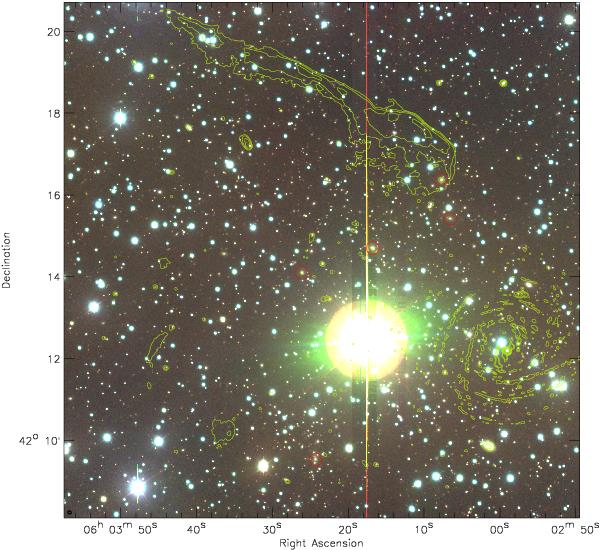
\includegraphics[width=0.5\textwidth]{toothbrush}
\end{figure}
\renewcommand{\baselinestretch}{2}

Optical data for the Toothbrush Cluster were taken in the VRI bands (V: 5510\AA, R: 6580\AA, I: 8060\AA) using the 4.2m William Herschel telescope (WHT) at Leiden Observatory in the Netherlands. (van Weeren et al. 2012 \cite{reinout12}) Radio data were taken at the Westerbork Synthesis Radio Telescope (WSRT, also at Leiden Observatory) and the Giant Metrewave Radio Telescope (GMRT, at the Tata Institute of Fundamental Research in India), for wavelengths ranging from 147 MHz to 4.9 GHz. (van Weeren et al. 2012 \cite{reinout12}) In order to determine the distribution of the intracluster gas, x-ray data were obtained from the ROSAT All-Sky Survey. 

\renewcommand{\baselinestretch}{1}
\begin{figure}[h]
\caption{X-ray and radio data for the Toothbrush Cluster. Orange denotes the x-ray taken from the ROSAT All-Sky Survey; black contours denote the radio from WSRT. Figure from van Weeren et al. (2012) \cite{reinout12}.}
\label{toothbrush_radio}
\centering
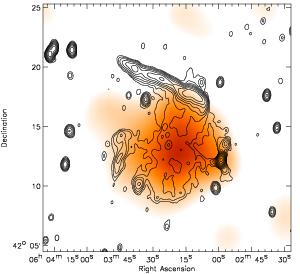
\includegraphics[width=0.5\textwidth]{toothbrush_radio}
\end{figure}
\renewcommand{\baselinestretch}{2}

A follow-up study was conducted by Will Dawson in January 2013, using two masks of the DEep Imaging Multi-Object Spectrograph (DEIMOS) at the W. M. Keck Observatory in Hawaii to spectroscopically identify galaxy redshifts and confirm their membership in the Toothbrush Cluster. 130 cluster members were confirmed (Figure \ref{velocities}), a large enough sample to begin applying statistical methods to the analysis of these cluster members' velocities and the overall properties of the merger. 

\renewcommand{\baselinestretch}{1}
\begin{figure}[h]
\caption{The redshifts of galaxies studied in the DEIMOS spectroscopic observation. Most of the galaxies fall in the Toothbrush Cluster, as evidenced by the peak around z=0.23. This peak is somewhat bimodal, lending further credence to the conclusion that there are multiple subclusters within the Toothbrush merger. Figure courtesy of Will Dawson.}
\label{velocities}
\centering
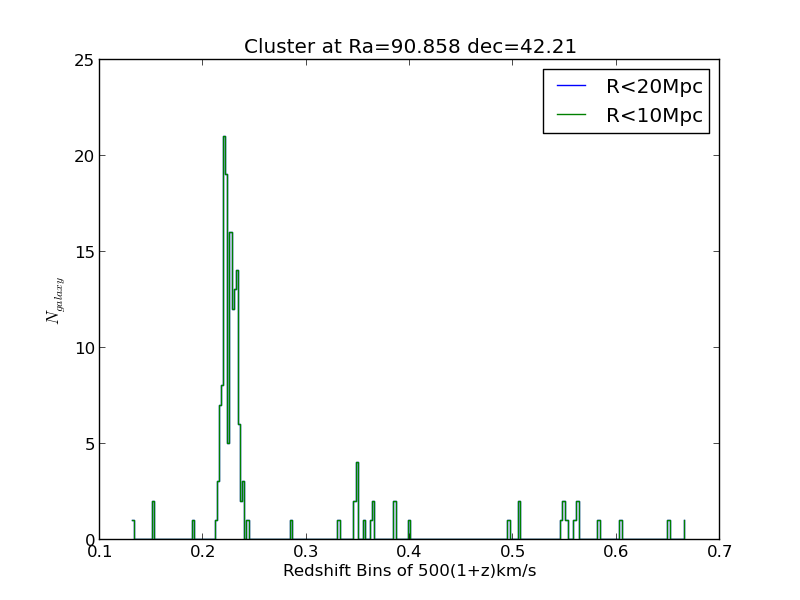
\includegraphics[width=0.8\textwidth]{hist_allspec}
\end{figure}
\renewcommand{\baselinestretch}{2}

\subsection{Bayesian Framework: MCMAC and Polarization Constraint Code}

To analyze these data, the Monte Carlo Merger Analysis Code (MCMAC) written by Dawson (2012) was used to simulate parameters of the galaxy cluster merger and determine the likelihood of each of the subsequent models \cite{Dawson13}. Observational data from the 2013 spectroscopic study of the Toothbrush Cluster were used to estimate the subclusters' masses, redshifts, and projected separation distance. These values were then used as inputs into the code, which assumed a Gaussian distribution around the inputs and then drew random values from the parameter distributions to create a possible model for the cluster's behavior (Figure \ref{willfig}). 

\renewcommand{\baselinestretch}{1}
\begin{figure}[h]
\caption{The basic geometry of the system. The mergers have some line-of-sight distance ($d_{proj}$) and velocity ($v_{rad}$) relative to each other, which is a component of their relative three-dimensional distance ($d_{3d}$) and velocity ($v_{3d_{obs}}$). The merger axis is at an angle $\alpha$ with the horizontal. Figure from Dawson (2012) \cite{Dawson13}.}
\label{willfig}
\centering
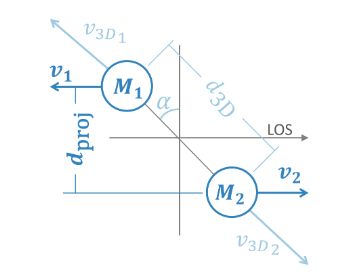
\includegraphics[width=0.5\textwidth]{willfig}
\end{figure}
\renewcommand{\baselinestretch}{2}

The code assumes that rather than behaving as point masses or uniform spheres, the subclusters behave as Navarro-Frenk-White dark matter halos (ie, they have a distribution that fits the form 

\renewcommand{\baselinestretch}{1}
\begin{equation}
\label{nfw}
\rho(r) = \frac{{\rho}_0}{\frac{r}{R_s} (1+\frac{r}{R_s})^2},
\end{equation}
\renewcommand{\baselinestretch}{2}

where $R_s$ and ${\rho}_0$ are specific to each dark matter halo). Each of these models displays six different input parameters (Table \ref{tab3}) and nine output parameters (Table \ref{tab4}), and assigns a probability of the system's occurring given observational data as a prior. 

\renewcommand{\baselinestretch}{1}
\begin{table}
\begin{tabular}{|p{1.75in}|p{4in}|} \hline
\textbf{Input Parameter Name} & \textbf{Input Parameter Description} \\ \hline
$m_1$ & The mass of the first subcluster ($10^{14} M_{\odot}$) \\ \hline
$m_2$ & The mass of the second subcluster ($10^{14} M_{\odot}$) \\ \hline
$z_1$ & The redshift of the first subcluster \\ \hline
$z_2$ & The redshift of the second subcluster \\ \hline
$\alpha_{out}$ & The viewing angle of the system, from the merger axis to the horizontal ($^{\circ}$) \\ \hline
$d_{proj}$ & The projected distance between the centers of the subclusters, at time of observation (Mpc) \\ \hline
\end{tabular}
\caption{The input parameters of the MCMAC code, with descriptions.}
\label{tab3}
\end{table}
\renewcommand{\baselinestretch}{2}

\renewcommand{\baselinestretch}{1}
\begin{table}
\begin{tabular}{|p{1.75in}|p{4in}|} \hline
\textbf{Output Parameter Name} & \textbf{Output Parameter Description} \\ \hline
$d_{3d}$ & The three-dimensional distance between the subcluster centers at time of observation (Mpc) \\ \hline
$d_{max}$ & The maximum distance between subcluster centers in the system (Mpc) \\ \hline
$v_{rad}$ & The relative observed velocity of the subclusters, at time of observation (km/s) \\ \hline
$v_{3d_{obs}}$ & The relative three-dimensional velocity of the subclusters, at time of observation (km/s) \\ \hline
$v_{3d_{col}}$ & The relative three-dimensional velocity of the subclusters, at time of collision (km/s) \\ \hline
$TSM_0$ & The time between collision and the system\'s observed state (assuming outbound) (Gyr) \\ \hline
$TSM_1$ & The period of the system (Gyr) \\ \hline
$T$ & The time between collision and the system\'s observed state (assuming outbound) (Gyr) \\ \hline
prob\_out & The probability that a model system with parameter values assigned by MCMAC is consistent with the observed system \\ \hline
\end{tabular}
\caption{The output parameters of the MCMAC code, with descriptions.}
\label{tab4}
\end{table}
\renewcommand{\baselinestretch}{2}

However, the Monte Carlo Merger Analysis Code (MCMAC) does not take into account the radio data. To use radio data as a prior, it was necessary to determine how the data could constrain one of the system parameters, in order to more effectively limit the number of possible merger models. Ensslin et al. (1998) provided a theoretical basis for constraining the viewing angle of the system given the polarization of that merger \cite{Ensslin98}. As discussed in Section 2.2, the polarization fraction of the system can be strongly related to whether the system is being viewed edge-on or face-on. However, this  relationship is complicated somewhat by magnetic field strength. Depending on many merger properties, the magnetic field outside the merger may be strong and very ordered or weak and very disordered. In the former case, the polarization fraction (which depends strongly on the degree of organization of the magnetic field) may have a high maximum value, while in the latter case, the maximum polarization fraction could be nearly zero (see Figure \ref{ensslin}).

\renewcommand{\baselinestretch}{1}
\begin{figure}[h]
\caption{The relationship between fractional polarization and viewing angle, with weak (dotted line) and strong (solid line) magnetic fields. The upper pair of lines are calculated with a spectral index of 1, while the lower pair of lines are calculated with a spectral index of 1.5 (see Equation \ref{strongfield}). Note that Ensslin et al. defined viewing angle as being angle between merger axis and the line of sight, while Dawson (2012) defined viewing angle as being between merger axis and the horizontal (Figure \ref{willfig}). These differences were taken into account in the analysis, and final results are shown according to the geometry used by Dawson \cite{Dawson13}. Figure from Ensslin et al. (1998) \cite{Ensslin98}.}
\label{ensslin}
\centering
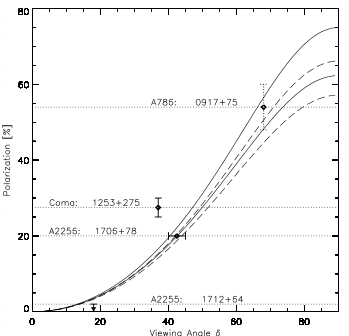
\includegraphics[width=0.5\textwidth]{ensslin_curves}
\end{figure}
\renewcommand{\baselinestretch}{2}

In order to account for this, Ensslin et al. modeled both the strong magnetic field and the weak magnetic field cases in determining a relationship between viewing angle and polarization fraction, and discovered that for a given polarization, a strong magnetic field provided the most conservative constraint on the viewing angle. As a result, I used the strong field theoretical relationship, 

\renewcommand{\baselinestretch}{1}
\begin{equation}
\label{strongfield}
<P_{strong}> = \frac{\gamma + 1}{\gamma + \frac{7}{3}} \frac{sin^2 \delta}{\frac{2}{15} \frac{13R-7}{R-1} -sin^2 \delta},
\end{equation} 
\renewcommand{\baselinestretch}{1}

as the basis for my code that constrained models of the viewing angle with the polarization fraction. (Note that $\gamma = 2\alpha_{spec} + 1$ is the spectral index of the electrons, $\alpha_{spec}$ is the spectral index of the radio emission, $R=\frac{\alpha + 1}{\alpha - \frac{1}{2}}$ is the shock compression ratio.)

Polarization and spectral index values for the toothbrush cluster were taken from the radio data published by van Weeren et al. (2012) Values for the polarization fraction of the radio relic varied between 10\% and 60\%; however, average values fell between 15\% and 30\%. For this model, I chose to use three values for the polarization fraction as constraints on the system: the minimum possible initial polarization value (0\%), the maximum value (60\%, as determined from the radio data), and a likely average value (20\%). These values were then used to calculate the likelihood (evidence) in the Bayesian analysis, and nineteen million MCMAC-generated probabilities associated with certain model viewing angles were used as the priors.

For each model viewing angle, I calculated the expected polarization fraction of an associated radio relic based on Equation \ref{strongfield}. I then used Bayes' Theorem (Equation \ref{bayes}) to find the probability that each model matched the data. If the expected polarization fraction value was found to be within the constraint, the likelihood was given a value of 1. However, if the expected polarization fraction was outside the constraint, the likelihood was assigned by determining the number of standard deviations between the constraint and the polarization fraction and calculating the probability that such a polarization fraction would be obtained. From there, the calculated likelihood was then multiplied by the prior probability to find a new probability that the system would be observed at that model's viewing angle. In this manner, each model was described by a probability of being valid, and could thus be compared to other randomly-generated models. After repeating this procedure for each of the models, the new credible region of the model was determined and plotted on a two-dimensional histogram for each parameter.

\newpage
\section{Results}

The parameter of most interest in constraining dynamical properties of a dissociative merger system (eg., the time since collision, the velocity of each subcluster at impact, the three-dimensional distance between the subcluster centers) is the viewing angle, $\alpha$. Indeed, the Toothbrush cluster displays changes to the credibility region of the values of these dynamical parameters due to the radio polarization fraction constraints on the viewing angle. 

The viewing angle of the Toothbrush Cluster did not significantly constrain the mass or redshift of either subcluster, or the projected distance between the subclusters. Since these values were used as inputs into the Monte Carlo code and were thus fairly well-defined, this result is consistent with expectations. On the other hand, limiting the viewing angle added a tight constraint on the three-dimensional distance between the subcluster centers – as evidenced in Figure \ref{mass}, with no viewing angle constraint, possible three-dimensional distance values ranged between 0 Mpc and 14 Mpc, while a polarization constraint of only 20\% limited the subclusters to being under 4 Mpc from each other at the time of observation, and a 60\% constraint limited them to being under 2 Mpc separated (Figure \ref{d3d}). 

\renewcommand{\baselinestretch}{1}
\begin{figure}[h]
\caption{Mass of the first subcluster. Blue regions indicate no polarization constraint, red regions indicate a 20\% constraint, and green regions indicate a 60\% constraint. Inner curves indicate a 95\% confidence region, and outer curves a 68\% confidence region. Note that the constraint on viewing angle did not change the range of mass values substantially.}
\label{mass}
\centering
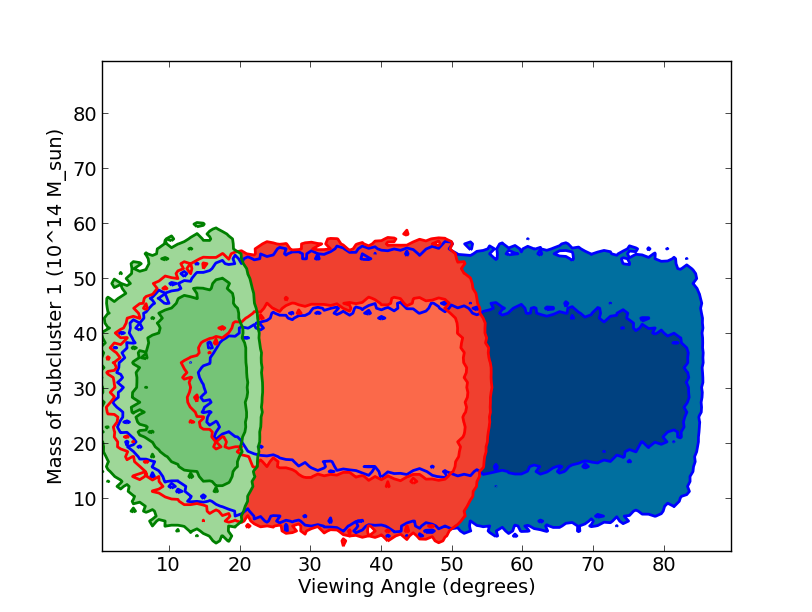
\includegraphics[width=0.5\textwidth]{alpha_m_1}
\end{figure}
\renewcommand{\baselinestretch}{2}

\renewcommand{\baselinestretch}{1}
\begin{figure}[h]
\caption{Observed 3D distance between the subclusters. As with the previous figure, blue regions indicate no polarization constraint, red regions indicate a 20\% constraint, and green regions indicate a 60\% constraint. Inner curves indicate a 95\% confidence region, and outer curves a 68\% confidence region.}
\label{d3d}
\centering
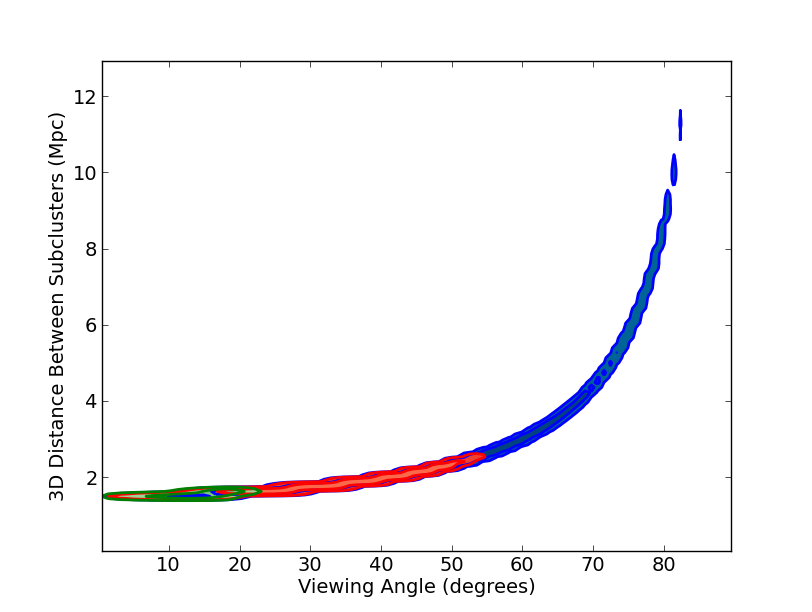
\includegraphics[width=0.5\textwidth]{alpha_d_3d}
\end{figure}
\renewcommand{\baselinestretch}{2}

Interestingly, 3D velocity at the time of collision was constrained slightly further (Figure \ref{velcol}), but the constraint on 3D velocity at the time of observation was slightly loosened, as evidenced by Figure \ref{velobs}. 

\renewcommand{\baselinestretch}{1}
\begin{figure}[h]
\caption{3D collision velocity of the subclusters.}
\label{velcol}
\centering
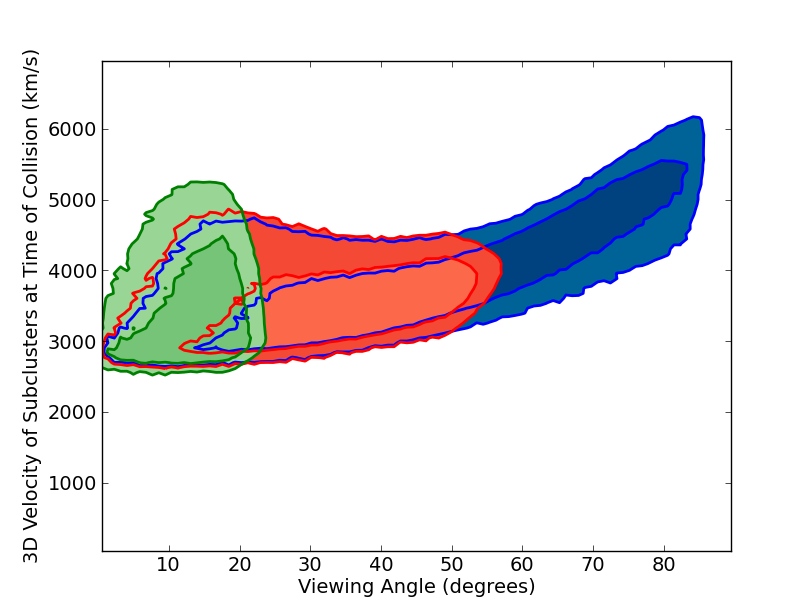
\includegraphics[width=0.5\textwidth]{alpha_v_3d_col}
\end{figure}
\renewcommand{\baselinestretch}{2}

\renewcommand{\baselinestretch}{1}
\begin{figure}[h]
\caption{Observed 3D velocity between subclusters.}
\label{velobs}
\centering
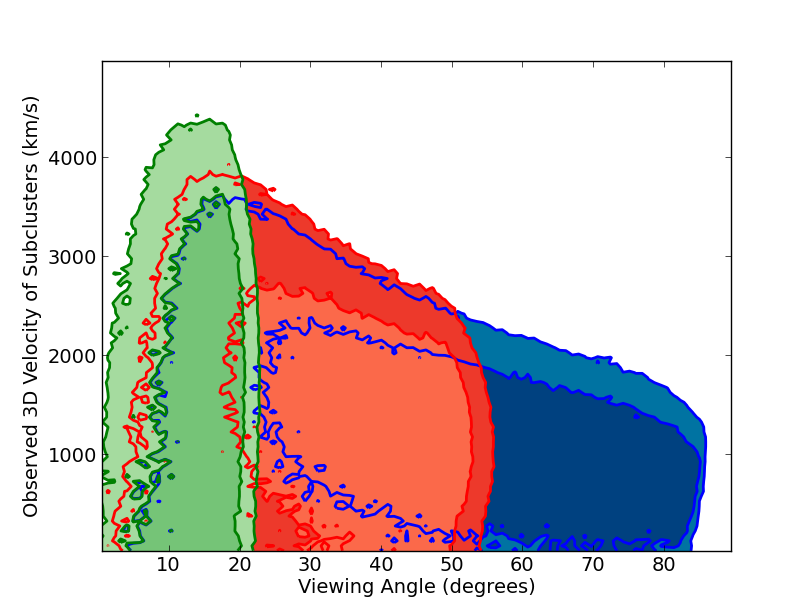
\includegraphics[width=0.5\textwidth]{alpha_v_3d_obs}
\end{figure}
\renewcommand{\baselinestretch}{2}

Since observed 3D velocity is comprised of the projected 2D velocity between subclusters:

\renewcommand{\baselinestretch}{1}
\begin{equation}
\label{veq}
v_{3d_{obs}} = v_{rad} / sin(\alpha),
\end{equation}
\renewcommand{\baselinestretch}{2}

it makes sense that in the limit where $\alpha \rightarrow 0 $, the observed 3D velocity would become more uncertain. Although this effect occurs in calculating the 3D velocity at time of collision, the decrease in the number of possible values for alpha was large enough that the range of probable 3D collision velocity values was able to be constrained by the analysis (albeit by only a very small amount). 

Since we can only observe this system as a static two-dimensional projection, it is possible that the system could be in one of multiple stages of the merger. After the initial collision, the two groups of dark matter and galaxies move away from the center of the merger until they have reached their maximum distance from each other and fall back toward the center of the potential, where they merge again. The time between the initial collision and the second collision is given by the period, 

\renewcommand{\baselinestretch}{1}
\begin{equation}
\label{T}
T=2 \int_0^{d_{max}} \frac{dr}{\sqrt{\frac{2}{\mu} (E-V(r))}},
\end{equation}
\renewcommand{\baselinestretch}{2}

which is derived in Dawson (2012) \cite{Dawson13}. Thus, two solutions for time since collision were analyzed: a solution in which the system is still traveling away from the center of the merger (outbound solution) and one in which the system is traveling back toward the center of the merger (inbound solution).  The possible values for the period were also analyzed.

\renewcommand{\baselinestretch}{1}
\begin{figure}[h]
\caption{Period between collisions.}
\label{period}
\centering
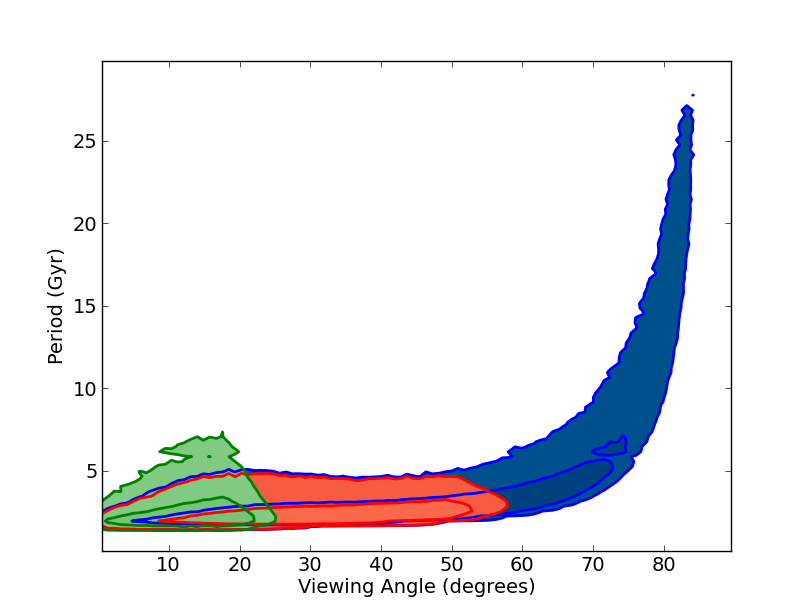
\includegraphics[width=0.5\textwidth]{alpha_T}
\end{figure}
\renewcommand{\baselinestretch}{2}

The credible region for the period of the system between collisions shrank as a result of adding a polarization prior, from 1-28 Gyr with no prior to 1-5 Gyr with a 20\% polarization fraction and 1-8 Gyr with a 60\% polarization fraction (Figure \ref{period}. Nevertheless, as evident in Figure \ref{TSM0}, the outbound solution for time since merger was also well-constrained with this analysis, with a 20\% constraint limiting the system to within 1.5 Gyr of collision (rather than the up to 8 Gyr possible with no constraint). After a 20\% constraint, however, constraining the system further led to very little decrease in the probability distribution of the time since collision.

\renewcommand{\baselinestretch}{1}
\begin{figure}[h]
\caption{Time since merger, outbound solution.}
\label{TSM0}
\centering
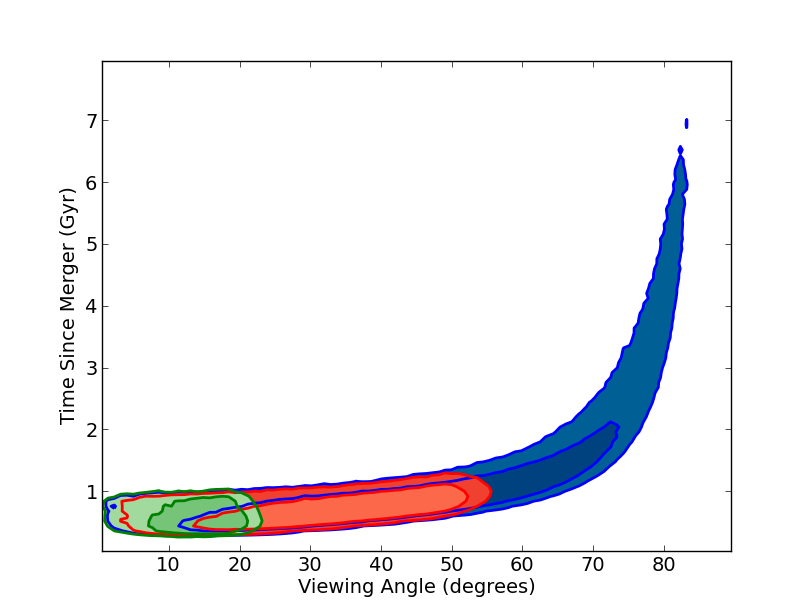
\includegraphics[width=0.5\textwidth]{alpha_TSM_0}
\end{figure}
\renewcommand{\baselinestretch}{2}

For the inbound solution, without any polarization constraint, time since merger could have had any value from 0.5 Gyr to 20 Gyr. With a 20\% constraint, this range decreased to 0.5 Gyr to 4.5 Gyr, and with a 60\% polarization fraction, the range widened a bit (Figure \ref{TSM1}. It is likely that the wider ranges for the period between collisions and the time since collision for the inbound solution occur as a result of constraining $\alpha$ to be closer to zero. Time since collision and period depend on the 3D velocity between subclusters, which becomes more uncertain with a viewing angle constrained closer to zero. 

\renewcommand{\baselinestretch}{1}
\begin{figure}[h]
\caption{Time since merger, inbound solution.}
\label{TSM1}
\centering
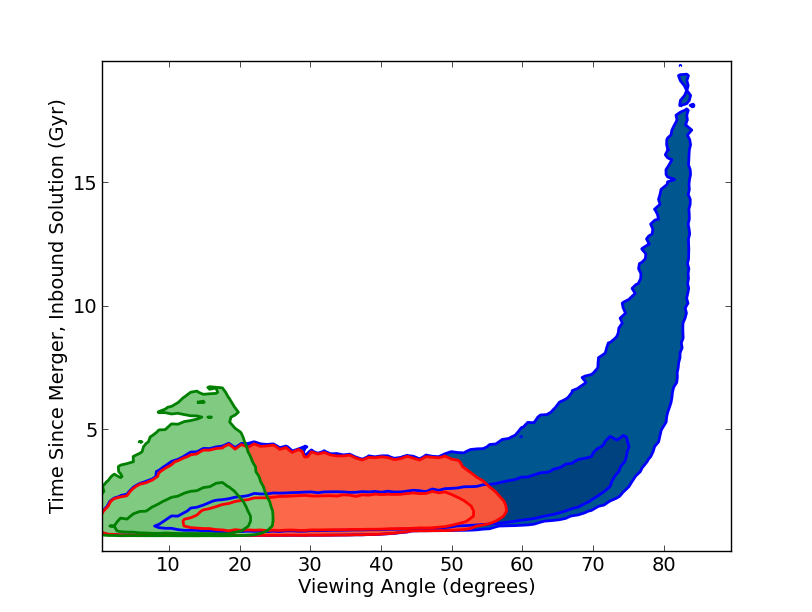
\includegraphics[width=0.5\textwidth]{alpha_TSM_1}
\end{figure}
\renewcommand{\baselinestretch}{2}

However, these increased uncertainties in the inbound solution are unlikely to greatly impact the model, since the inbound solution is somewhat less likely to model the system well. If the inbound solution were a likely model, the time since collision would have been substantially longer than that modeled by the outbound solution, and the Toothbrush Cluster radio relics would have probably traveled farther from the center of the cluster than observations of the actual system indicate. Nevertheless, the constraints on the solutions for the time since collision parameter were not strong enough to determine rigorously whether the inbound or the outbound solution is more likely to accurately model the behavior of the Toothbrush Cluster, since the credibility regions of each system overlapped enough that an analysis would be unable to differentiate between them in any significant manner. Given better data or stronger constraints, this analysis could be conducted more comprehensively and one of the two solutions could be ruled out.

\newpage
\section{Discussion and Future Work}

These results have demonstrated the power of a polarization fraction constraint in narrowing the range of possible values of other parameters, including viewing angle, time since collision, 3D velocity at time of collision, period between collisions, and observed 3D distance. It is reasonable that this should be so, since these parameters are not independent of each other. Some of the parameters (eg. observed 3D distance, observed 3D velocity) directly depend on the viewing angle (Equation \ref{veq}). Other parameters, such as period between collisions and time since collision, depend on each other (eg., Equation \ref{T}).

Although this method for constraining a merging galaxy cluster system's angle with the line of sight is clearly capable of substantially diminishing the credible region of the values of multiple merger parameters, it would benefit from being corroborated by other studies. Indeed, according to Equation \ref{bayes}, the posterior of this method may be considered a prior for another independent constraint, which would further diminish the credible region of likely parameter values for the Toothbrush Cluster merger. One such method is to use the relic distance from the cluster center to constrain its viewing angle. Radio relics cannot be formed at the center of a merger, since the gas is sufficiently dense that a disturbance in the molecules will move too quickly to produce a shock wave. At a certain distance from the merger center, the intracluster gas is not dense enough to allow a shock wave to continue to propagate. Thus, only in a fairly narrow region of the merger (0.5-1.5 Mpc) would it be possible to see radio relics emerge at all (van Weeren et al. 2011c \cite{reinout11c}, Vazza et al. 2011 \cite{Vazza11}). Vazza et al. (2011) have used this method to constrain the viewing angle based on the position of the radio relic relative to the narrow range of allowed positions \cite{Vazza11}.

A similar but independent method is to constrain the time since collision using the position of the radio relic and a model of the velocity of the relic. Since

\renewcommand{\baselinestretch}{1}
\begin{equation}
\label{distance}
d_{3d} = v_{3d_{obs}}(t) \cdot TSM_0, 
\end{equation}
\renewcommand{\baselinestretch}{2}

if we know the distances at which we will most likely find the radio relic, the velocity of the relic and the time since merger can be constrained. The values of $TSM_0$ and $v_{3d_{obs}}$ can be used to calculate the expected position of the radio relic, since simulations suggest that the radio relic speed varies little with time and is very close to $v_{3d_{obs}}$. Additionally, with more detailed simulations of the gas density as a function of time, speed of sound could be determined more accurately; thus, a hydrodynamic simulation of the gas dynamics could prove to be a powerful complement to this approach.

Constraining the dynamics of merging systems has important implications in a variety of scientific pursuits. Dark matter searches, in particular, could benefit greatly from constraining the self-interaction cross-section of the elusive particles that comprise this material. Standard models of dark matter are based upon the premise that since dark matter-luminous matter interaction cross-section is extremely low, its self-interaction cross-section must be low as well; indeed, experiments that search for dark matter directly (eg. CDMS \cite{CDMS}, LUX \cite{LUX}, XENON \cite{XENON}, CoGeNT \cite{cogent}) and several indirect detection schemes focus on detecting dark matter that fits this standard description. However, as described in Section 2.1, galaxy cluster mergers show promise as laboratories in which to test whether dark matter may interact with itself more strongly than it interacts with luminous matter (some theorists do question the validity of using galaxy cluster mergers to test for SIDM, see Kahlhoefer et al. 2013 \cite{Kahlhoefer13}). With a smaller region of possible values that a model of the Toothbrush Cluster could take, it becomes possible to more effectively study this cluster, and studies seeking to constrain the self-interaction cross-section of dark matter could become more efficient in their modeling as a result. 

Finally, a study of the dynamical properties of this system could contribute greatly to an understanding of dissociative merging systems in general. There is currently no systematic way to identify galaxy cluster mergers – all mergers have been discovered by chance in large sky or cluster surveys. However, the exploration of radio-identified dissociative mergers could play a key role in changing that discrepancy. Because these radio relics are rarely seen apart from a galaxy cluster merger, it has been suggested that they may be used to identify possible dissociative merger systems (van Weeren et al. 2011b \cite{reinout11b}, c \cite{reinout11c}). In order to address that idea, this work could be used as part of a sample of radio-selected mergers to determine if these are likely to be dissociative, as well as investigating the properties of radio-selected mergers as compared to non-radio-selected mergers. 

\newpage
\section{Conclusion}

In this work, I have integrated radio data of the merging galaxy cluster 1 RXS J0603.3+4214 with probability distributions of merger parameters created with the Monte Carlo Merger Analysis Code (MCMAC) in order to determine new probability distributions for these parameters. I find that using the fractional polarization of the radio relics to constrain the viewing angle of the merger does put strong constraints on merger parameters such as the time since collision, 3D collision velocity, 3D observed distance, and period between collisions. These constraints can be used in a variety of future studies, particularly studies that work to constraint the self-interaction cross-section of dark matter.

\newpage
\section*{Acknowledgements}

I would like to express my gratitude to my thesis readers, David Wittman and Steve Naftilan, for their comments, insights, and guidance over the course of researching and writing this thesis. Thanks to Will Dawson for use of his MCMAC code, Toothbrush Cluster spectroscopic data, and wonderful advice. I am also grateful to the Keck Science Department of Scripps College and the UC Davis Cosmology group for being welcoming environments in which to conduct research. Thanks to Scot Gould, whose support and encouragement have been unwavering, and who first invited me to really take a look at physics (I've never looked back!) I thank Cameron Conti, Madeleine Bulkow, Simone Maule, and Matthew Lawson for their editing, suggestions, offers to edit, offers to let me use their computers, and late-night shenanigans, and for helping me to remain sane during this process. Finally, I wish to thank my family for their continued support of this thesis and of everything I do.

\newpage
\section*{Literature Cited}

\bibliography{cosmology}
\bibliographystyle{plain}

\newpage
\section*{Appendix}

This appendix contains the code used to constrain the viewing angle with the polarization fraction obtained from the radio relics.

\renewcommand{\baselinestretch}{1}
\begin{verbatim}

# EQ Finney
# Polarization Constraint Code

import math
import numpy
import pickle
import scipy.special as sci
import matplotlib.pyplot as plt

def exp_pfrac(delta, alpha):
    """ Determines fractional polarization expected from a model of given
        viewing angle and spectral index.
        Input:
        delta: the inclination angle provided by the model (in degrees)
        alpha: the spectral index as determined in the literature, used to
               calculate the expected polarization of a model viewed from a
               certain angle
        Output:
        pfrac_expected: the fractional polarization of the radio relic, as
                        determined by the relationship in Ensslin et al. 2008
    """
    Rexp = (alpha + 1)/(alpha - 0.5) # shock compression ratio
    gamma = 2*alpha + 1 # spectral index of the electrons

    # Calculating the strong field expected polarization
    gammacoeff = (gamma + 1)/(gamma + (7./3))
    ratioterm = ((2.0/15)*(13.0*Rexp-7)/(Rexp-1))
    deltarad = delta*math.pi/180.0
    angleterm = (math.sin(deltarad))**2
    pfrac_expected = gammacoeff*(angleterm/(ratioterm - angleterm))
    return pfrac_expected


def wlikelihood(pfrac_expected, pfrac, sigma):
    """ Given an expected fractional polarization and an array size and spacing,
        computes the value of the error function in a range around the expected
        value. Need to have a standard deviation value for this to work.
        Inputs:
        pfrac_expected: the fractional polarization of the radio relic, as
                        determined by the relationship outlined in Ensslin et
                        al. 2008 and carried out by the uwlikelihood function
                        above
        pfrac: the fractional polarization of the radio relic, as determined
               from the literature values
        sigma: the standard deviation of the fractional polarization
        Outputs:
        z: the number of standard deviations from the expected value to pfrac
        likelihood: the probability that pfrac is consistent with pfrac_expected
    """
    # This constraint is REALLY conservative.
    z = (pfrac_expected-pfrac)/sigma
    if (z>0):
        likelihood = 1
    else:
        #print "The number of standard deviations away is:", z
        likelihood = sci.erfc(math.fabs(z))
    return z, likelihood


def probability(delta, alpha, pfrac, sigma):
    """ Incorporates the above two functions into a main function that
        determines the likelihood of an inclination angle given how it compares
        to the expected fractional polarization.
        Inputs:
        delta: the inclination angle provided by the model (in degrees)
        alpha: the spectral index as determined in the literature, used to
               calculate the expected polarization of a model viewed from a
               certain angle
        pfrac: the fractional polarization of the radio relic, as determined
               from the literature values
        sigma: the standard deviation of the fractional polarization
    """
 
    # Checking to see if the parameters fit the code
    if (delta > 90) or (delta < 0):
        print "delta must be between zero and ninety degrees! Exiting."
        sys.exit()

    # Calculating the expected fractional polarization
    pfrac_expected = exp_pfrac(delta, alpha)
    
    # Calculating the likelihood of seeing this system given actual data
    z, likelihood = wlikelihood(pfrac_expected, pfrac, sigma)
    if (delta > 70):
        print "The inclination angle is:", delta
        print "The expected fractional polarization is:", pfrac_expected
        print "The actual fractional polarization is: ", pfrac
        print "The actual polarization is", z, "sigma from the expected value."
        print "The likelihood is:", likelihood
    return likelihood

def main(prob_MCMC, angle_MCMC, spectral_index, pfrac, sigma=0.05, prefix=''):
    """ Takes in Will's pickle files (which contain hundreds of MCMC results)
        and then for each result uses the angle from MCMAC to compute a
        likelihood (with radio prior) using my probability function. This is
        subsequently multiplied by the probability obtained from MCMAC to
        get an overall probability, which is written to pickle file for future
        use and plotting.
        Inputs:
        prob_MCMC: the name of a pickle file containing an array of
                   probabilities (string)
        angle_MCMC: the name of a pickle file containing an array of viewing
                   angles (string)
        spectral_index: the spectral index of the system as determined from
                   literature (float)
        pfrac: the polarization fraction of the system as determined from the
               literature (float)
        sigma: the standard deviation of the fractional polarization (float)
        prefix: a prefix of the pickle file to be written (float)
        No outputs, but an array of probabilities is written to file
    """

    # loading pickle arrays from file
    array_prob = pickle.load(open(prob_MCMC,'rb'))
    array_angle = pickle.load(open(angle_MCMC,'rb'))

    # Making certain that information is in the correct form
    if (spectral_index < 0):
        spectral_index = math.fabs(spectral_index)

    if (pfrac > 1) or (pfrac < 0):
        print "pfrac must be between 0 and 1! Exiting."
        sys.exit()

    # Running the actual code
    size = numpy.size(array_angle)
    mod_prob_array = numpy.zeros(size)
    init_prob_array = numpy.zeros(size)

    for index in range(size):
        # accounting for differences between Dawson 2012 and Ensslin 1998
        angle = (90 - array_angle[index])
        
        likelihood = probability(angle, spectral_index, pfrac, sigma)
        init_prob_array[index] = likelihood
        mod_prob_array[index] = likelihood*array_prob[index]

    # Then do something like pfrac vs. inclination angle, with different colors
    # for different likelihood values, and see where they fall.
    i = [(90-x) for x in array_angle]
    if numpy.size(i) == numpy.size(init_prob_array):
        plt.scatter(i,init_prob_array, marker='s')
        plt.title('Probability of system, given polarization')
        plt.xlim(0,90)
        plt.ylim(0,1)
        plt.xlabel('inclination angle')
        plt.ylabel('probability')
        plt.savefig(prefix+'_radio_fig.png')
        F = open(prefix + '_radio_fig.png')
        F.close()
        plt.close()
        
    filename = prefix+'_radio_prob.pickle'
    F = open(filename, 'w')
    pickle.dump(init_prob_array,F)
    F.close()
    filename = prefix+'_mod_prob.pickle'
    F = open(filename, 'w')
    pickle.dump(mod_prob_array,F)
    F.close()
    return

\end{verbatim}

\end{document}
